%%
%% ESEM 2026 Technical Track submission (DOUBLE-ANONYMOUS).
%% LIPIcs format, 17 pages main + up to 3 pages refs/data.
%% Compile: pdflatex -> bibtex -> pdflatex -> pdflatex
%%
%% Structured abstract required (Background/Aims/Method/Results/Conclusions).
%% Data Availability section is mandatory.
%%

\documentclass[a4paper,UKenglish,cleveref,autoref,thm-restate]{lipics-v2021}

%% --- packages ---
\usepackage{microtype}
\emergencystretch=2em
\usepackage{booktabs}
\usepackage{listings}
\usepackage{xcolor}
\usepackage{tikz}
\usetikzlibrary{positioning,arrows.meta,shapes.geometric,calc,fit}

\lstset{
  basicstyle=\ttfamily\footnotesize,
  keywordstyle=\color{blue!70!black}\bfseries,
  commentstyle=\color{green!50!black}\itshape,
  stringstyle=\color{red!60!black},
  showstringspaces=false,
  breaklines=true,
  frame=single,
  framesep=3pt,
  xleftmargin=4pt,
  aboveskip=4pt,
  belowskip=4pt,
  columns=flexible,
}

\lstdefinelanguage{OCL}{
  morekeywords={context,inv,pre,post,let,in,if,then,else,endif,
    self,implies,and,or,not,forAll,exists,select,collect,size,
    includes,oclIsKindOf,oclIsUndefined,oclAsType,Set,Bag,Sequence,Tuple,
    String,Integer,Boolean,SpanKind},
  sensitive=true,
  morecomment=[l]{--},
  morestring=[b]'
}

%% --- LIPIcs metadata (DOUBLE-ANONYMOUS submission) ---
\title{The Conformance Gap is a Framework Gap: An Empirical Survey of Six AI-Agent SDKs and a Controlled Telemetry Benchmark on 14 Fault Classes}

\titlerunning{The Conformance Gap is a Framework Gap}

%% Anonymized author block — populate only after acceptance.
\author{Anonymous Author(s)}{Anonymous Institution}{}{}{}
\authorrunning{Anonymous}

\Copyright{Anonymous}

\ccsdesc[500]{Software and its engineering~Software verification and validation}
\ccsdesc[300]{Software and its engineering~Software performance}
\ccsdesc[300]{Computing methodologies~Distributed artificial intelligence}

\keywords{AI agent observability, OpenTelemetry, fault detection, empirical software engineering, controlled experiment, telemetry metamodels}

\category{} %% Type of submission, leave empty for regular technical paper.

\relatedversion{} %% Filled in after acceptance / when an arXiv version exists.

\supplement{Replication package: see Data Availability statement (\S\ref{sec:data}).}
\supplementdetails[subcategory={Software, Dataset}]{Software}{Anonymized for review.}

\funding{} %% Anonymized.

\acknowledgements{} %% Anonymized.

\nolinenumbers

%% LIPIcs cleveref defaults
\hideLIPIcs

\begin{document}

\maketitle

%% =====================================================================
%% Structured abstract (Background / Aims / Method / Results / Conclusions)
%% =====================================================================
\begin{abstract}
\noindent\textbf{Background.} Three industry telemetry vocabularies---generic
OpenTelemetry, OpenTelemetry GenAI, and OpenInference---compete to
instrument autonomous AI-agent systems built on LLMs.  Production
agent stacks layer these conventions on top of framework SDKs
(LangChain, LlamaIndex, AutoGen, CrewAI, Anthropic SDK, OpenAI Agents)
whose default tracing emissions vary widely.  No prior empirical
study has measured how much of the observed cross-stack typed-capability
variance comes from metamodel choice versus per-framework
instrumentation defaults.

\noindent\textbf{Aims.} (RQ1) How does the typed-capability footprint
(TCR; FPR) of the three industry metamodels compare on a controlled
simulation benchmark of 14 agent-specific fault classes (12 of 14
MAST modes exercised; FM-1.2 and FM-2.2 omitted)? (RQ2) How much of
the realized cross-adapter variance is attributable to
framework-instrumentation defaults rather than metamodel design?
(RQ3) How sensitive are the measurements to detector thresholds, the
per-framework profile, and the foundation-model dimension?

\noindent\textbf{Method.} A controlled fault-injection harness
exercises 14 paired faults across 4 detector banks and 6 telemetry
conditions on 7 framework-adapter profiles whose per-kind coverage is
grounded in a direct survey of each SDK's source as of 2026-05
(pinned commit SHAs in \texttt{coverage\_matrix.md}); the adapters
are executable simulations, not live package integrations. Three
scoring rules---standardized-field, permissive substring, and
conformant extended-attribute dispatch restricted to attributes
\emph{actually published} in each metamodel---are reported in
parallel. Inferential units are $n = 14$ paired faults and $G = 6$
third-party adapter clusters; we lead with small-$G$-appropriate
inference (cluster bootstrap, cluster-level $t$ test at $G - 1 = 5$ df, and a
fault-cluster sign-flip permutation) and report asymptotic GEE as
sensitivity. 13 of 14 faults map
onto MAST modes \cite{anon-mast} and were re-coded by a second
annotator (Cohen's $\kappa = 0.83$, bootstrap 95\% CI $[0.58, 1.00]$);
a Domain-Specific Metamodel (DSM) authored by us is included as a
uniformly-applied measurement instrument.

\noindent\textbf{Results.} \emph{Framework-instrumentation defaults
drive the largest observed spread.} Per-adapter realized DSM TCR ranges
$4.5\times$, from $2/14 = 0.143$ on Anthropic SDK (no built-in
tracing) to $9/14 = 0.643$ on OpenAI Agents SDK (typed
\texttt{handoff} and \texttt{guardrail.triggered}); the four
remaining frameworks fall between. \emph{Live-LLM sanity check.}
In a cached live-CLI check ($90$ attempts; $88$ parsed; $82$
fault-bearing), LLM self-detection reaches $15/82 = 0.183$
(Wilson 95\% CI $[0.114, 0.280]$) with $0/6$ false alarms,
underscoring that self-report and telemetry measure complementary
surfaces. \emph{Cross-adapter inference is inconclusive at the
realized level.} The per-adapter $\Delta$TCR vector for DSM minus
OpenInference extended-attribute scoring is
$\{0, 0, 0, 0, 0, +2/14\}$: five of six third-party adapters yield
exact equivalence, with the $+2/84 = +0.024$ mean driven entirely
by OpenAI Agents SDK. The fault-cluster sign-flip permutation
gives two-sided $p = 0.75$; cluster bootstrap percentile 95\% CI
is $[0.000, +0.071]$; cluster-level $t$ test at $G - 1 = 5$ df two-sided $p =
0.36$ (asymptotic GEE-on-adapter $p = 0.264$ is sensitivity only at
$G = 6$). The 13-fault MAST-only sub-analysis yields the same
direction and magnitude ($+2/78 = +0.026$). OTel GenAI extended
attributes reach $38/84$ and an OpenInference EVALUATOR/PROMPT
counterfactual reaches $40/84$, both at zero FPR, so the DSM is not
a deployable recommendation. On the eight production-plausible
non-oracle faults, OpenInference extended is $23/48$ and DSM is
$24/48$ (default FPR $4/72$, threshold-tuned $0/72$); a supplemental
six-workflow no-fault suite selects the same tuned threshold with
held-out FPR $0/216$ and TP $60/72$. \emph{Designed
measurement spread.} The capability envelope ($14/14$ vs.\ $6/14$)
is the deterministic outcome the design produces and is reported
descriptively, not as inferential evidence.

\noindent\textbf{Conclusions.} The actionable open work for an SRE
today is per-framework instrumentation completeness, not metamodel
extension: OpenAI Agents SDK already saturates 5/9 typed kinds with
\texttt{handoff} and \texttt{guardrail.triggered}; Anthropic SDK
emits no built-in tracing. The methodological contribution is TCR
scored under conformant attributes, with per-framework coverage
cited against pinned SDK revisions and applied uniformly to four
metamodels; the stronger baseline counterfactuals are explicitly
reported, and the DSM is a measurement instrument, not a recommendation.
\end{abstract}

%% =====================================================================
\section{Introduction}
\label{sec:intro}

Autonomous agents built on large language models (LLMs) increasingly
execute production workflows in customer support, code review, and
incident response \cite{anon-langchain,anon-crewai,anon-autogen}.
Unlike traditional software, agents operate through stochastic loops
of \emph{planning}, \emph{tool execution}, \emph{reasoning}, and
\emph{delegation}.  As they enter production, observability has
become critical, and a growing empirical body shows that multi-agent
failures are dominated by agent-specific pathologies---specification,
inter-agent misalignment, and task verification---rather than the
network errors that dominate microservice incidents
\cite{anon-mast}.

The de-facto industry standard for distributed tracing,
OpenTelemetry (OTel), defines a metamodel for spans whose
\texttt{SpanKind} enumeration (\texttt{CLIENT}, \texttt{SERVER},
\texttt{INTERNAL}, \texttt{PRODUCER}, \texttt{CONSUMER}) was designed
for microservices.  Two AI-specific extensions have emerged:
OpenTelemetry GenAI \cite{anon-otelgenai} introduces typed operation
names including \texttt{create\_agent}, \texttt{invoke\_agent},
\texttt{execute\_tool}, and \texttt{retrieval}; OpenInference
\cite{anon-openinference} introduces ten typed span kinds including
\texttt{AGENT}, \texttt{GUARDRAIL}, \texttt{RETRIEVER}, and
\texttt{TOOL}.  Both narrow the gap relative to vanilla OTel.
Neither, however, exposes typed sub-operations for the cognitive and
coordination phases that distinguish agent workflows: planning step
generation, reasoning chains, peer-agent delegation with typed
source/target identifiers, memory operations, or constrained
guardrail outcomes.

This paper poses an empirical question that has not been answered in
prior work: \emph{how much of the observed cross-stack agent-fault
detection variance is attributable to metamodel choice versus
per-framework instrumentation defaults?}  We construct a controlled
fault-injection harness, adopt the multi-agent failure taxonomy
(MAST) of an independent prior team \cite{anon-mast} as
externally-anchored ground truth, and survey the default tracing
emissions of six AI-agent framework SDKs as of 2026-05 with
pinned source-survey evidence for each SDK. We then measure Typed
Capability Rate (TCR) and False-Positive Rate (FPR) under three
scoring rules: standardized-field dispatch, permissive substring
matching on surveyed default span names, and extended-attribute
dispatch restricted to attributes \emph{actually published} in each
metamodel's specification.

\paragraph*{What this paper does \emph{not} claim.}
The DSM under study was designed by us to add typed kinds for the
five phases the industry baselines omit, so the capability-envelope
gap is a quantification of a designed gap on a uniform measurement
instrument, not an empirical surprise. Our contribution is the
\emph{realized} measurement: per-framework coverage grounded in a
direct survey of each SDK's source, scoring restricted to attributes
actually published in each metamodel's convention, and uniform
application across all four metamodels. We do \emph{not} claim
generalization beyond the surveyed framework versions, the 14-fault
MAST-anchored taxonomy, the mocked LLM clients, or the three scoring
rules; we discuss scope explicitly in \Cref{sec:threats}.

\paragraph*{Contributions.}
This is a measurement-methodology paper whose central empirical
finding is that the realized cross-adapter spread induced by
surveyed framework instrumentation defaults ($4.5\times$ range,
$0.143$ to $0.643$) is much larger than the realized DSM-vs-baseline
metamodel contrast ($+0.024$ vs.\ OpenInference extended). Once
baseline detectors are restricted to
attributes actually published in the OpenInference and OTel GenAI
conventions, the realized DSM offers no statistically detectable
cross-adapter advantage under small-$G$-appropriate inference
(cluster bootstrap on per-adapter mean $\Delta$ percentile 95\% CI
$[0.000, +0.071]$; cluster-level $t$ test at $G - 1 = 5$ df two-sided $p = 0.36$;
sign-flip permutation two-sided $p = 0.75$). The DSM's capability
envelope advantage ($14/14$ vs.\ $6/14$) is a designed structural
property and is reported descriptively, not as inferential evidence.
\begin{enumerate}[(C1)]
\item A \textbf{framework-instrumentation reframing}: the realized
  cross-adapter range is driven by per-framework default emissions;
  OpenAI Agents SDK reaches $9/14 = 0.643$ realized DSM
  TCR (typed \texttt{handoff}, \texttt{guardrail.triggered}),
  Anthropic SDK $2/14 = 0.143$ (no built-in tracing).
\item A \textbf{survey-grounded apparatus}: per-profile DSM-kind
  coverage grounded in a direct survey of each SDK's source as of
  2026-05 (pinned commit SHAs in \texttt{coverage\_matrix.md}); 14
  faults (13 mapped onto MAST, $\kappa = 0.83$ bootstrap CI
  $[0.58, 1.00]$; 1 independently motivated) across 4 detector
  conditions $\times$ 7 adapter profiles $\times$ 6 mocked models
  $\times$ 2 privacy levels ($3{,}780$ rows; informative $n = 14$
  paired faults, $G = 6$ third-party adapter clusters).
\item \textbf{Three uniform scoring rules} (standardized-field,
  permissive substring on surveyed default span names,
  extended-attribute dispatch restricted to attributes \emph{actually
  published}) applied uniformly across all four metamodels.
\item A \textbf{small-$G$-appropriate statistical audit}: cluster
  bootstrap on $G = 6$ adapters and cluster-level $t$ test at $G - 1 = 5$ df as
  primary realized inference (per Cameron--Miller~\cite{cameron2015});
  sign-flip permutation as cluster-free alternative; asymptotic
  GEE as sensitivity; Wilson and Newcombe CIs; production-
  plausible non-oracle subset reported as the operational analysis;
  the 13-fault MAST-only sub-analysis matches the direction;
  detectable-significance floor at $n = 14$.
\item A \textbf{design-frozen, bit-for-bit-reproducible methodology}:
  workload $\to$ taxonomy $\to$ DSM $\to$ detector freeze;
  second-annotator MAST mapping; three predicate banks released;
  full matrix reproducible on a single CPU in $<3$ minutes.
\end{enumerate}

%% =====================================================================
\section{Background}
\label{sec:background}

\subsection{The OpenTelemetry Span Metamodel}

OpenTelemetry defines a span as the basic unit of execution in a
distributed trace, carrying a name, typed \texttt{SpanKind}, parent
reference, timestamps, status, attributes, events, and a
\texttt{Baggage} map propagated by W3C Trace Context
\cite{anon-w3ctrace}.  The five canonical \texttt{SpanKind} literals
(\texttt{CLIENT}, \texttt{SERVER}, \texttt{INTERNAL},
\texttt{PRODUCER}, \texttt{CONSUMER}) were designed for
microservice request--response interactions.

\subsection{The Two AI-Specific Conventions}

\paragraph*{OpenTelemetry GenAI semantic conventions.}
\cite{anon-otelgenai} adds a \texttt{gen\_ai.operation.name}
attribute with values including \texttt{chat},
\texttt{create\_agent}, \texttt{invoke\_agent},
\texttt{execute\_tool}, \texttt{retrieval}, \texttt{embeddings};
plus a small attribute namespace
(\texttt{gen\_ai.usage.\{input,output\}\_tokens},
\texttt{gen\_ai.tool.name}, \texttt{gen\_ai.agent.\{id,name\}}).

\paragraph*{OpenInference.}  \cite{anon-openinference} defines
\texttt{openinference.span.kind} with ten typed values:
\texttt{LLM}, \texttt{EMBEDDING}, \texttt{CHAIN}, \texttt{RETRIEVER},
\texttt{RERANKER}, \texttt{TOOL}, \texttt{AGENT}, \texttt{GUARDRAIL},
\texttt{EVALUATOR}, \texttt{PROMPT}; plus free-form attributes
(\texttt{tool.name}, \texttt{retrieval.documents}, etc.).

\subsection{The Coverage Gap and the MAST Taxonomy}

Both AI-specific conventions provide typed entities for the
\emph{visible} surface of an agent (LLM call, tool execution,
retrieval, agent lifecycle) but neither exposes typed sub-operations
for the \emph{cognitive} (planning, reasoning), \emph{coordination}
(peer-agent delegation with typed identifiers, memory), or
\emph{policy} (constrained guardrail outcomes) surfaces.  An
independent prior team \cite{anon-mast} presents the Multi-Agent
System Failure Taxonomy (MAST), classifying failures into 14 modes
across system design (FM-1.1--FM-1.5), inter-agent misalignment
(FM-2.1--FM-2.6), and task verification (FM-3.1--FM-3.3).  We adopt
MAST as the externally defined reference taxonomy against which our
fault-injection benchmark is mapped (\Cref{sec:taxonomy}).

\paragraph*{Positioning relative to prior tracing and empirical-SE work.}
The OpenTelemetry metamodel inherits a long line of distributed-tracing
systems (Dapper~\cite{anon-dapper}, Canopy~\cite{anon-canopy}, Pivot
Tracing~\cite{anon-pivottracing}); subsequent work addresses scalable
sampling~\cite{anon-sifter}, root-cause attribution~\cite{anon-xray},
and trace-analysis surveys~\cite{anon-tracingsurvey}. None addresses
the typed-semantic-convention question for autonomous agents.
Methodologically we follow empirical-SE conventions for controlled
experiments and case studies \cite{anon-wohlin,anon-runeson}: a
pre-frozen workload\,$\to$\,taxonomy\,$\to$\,DSM\,$\to$\,detector
design, externally anchored MAST labels, and per-fault-class binary
detection (cf.\ rule-based event-log analyses~\cite{anon-cinque})
within the runtime-verification frame~\cite{anon-rv}.

%% =====================================================================
\section{Method}
\label{sec:method}

\subsection{Research Questions}

\begin{itemize}
\item[\textbf{RQ1}] How does the typed-capability footprint
(TCR/FPR) of the three industry telemetry metamodels compare on a
controlled simulation benchmark of 14 agent-specific fault classes
under standardized-field dispatch? (Descriptive characterization;
the $n = 14$ design has Holm-3 detectability floor $\Delta_{\min} =
0.50$, so we do not attempt a high-resolution inferential test on
this contrast and report Wilson CIs and the exact range only.)
\item[\textbf{RQ2}] To what extent does a DSM that adds typed
sub-operations for delegation, planning, reasoning, guardrails, and
memory expand the typed-capability envelope relative to the industry
baselines, and how does the gap survive the obvious
counter-experiments---specifically (a)~a permissive substring-matching
scoring rule that lifts the baselines and (b)~per-adapter
implementation variance characterized by Wilson CIs and the exact
small-cluster adapter range?
\item[\textbf{RQ3}] How sensitive are the typed-capability
measurements to the detector-threshold dimension (characterized by a
threshold sweep on the only non-zero-FPR detector and a
train/held-out no-fault workflow check), the per-framework adapter
dimension (Wilson CIs per adapter, exact across-adapter range), and
the foundation-model dimension
(deterministic-replication sanity check)?
\end{itemize}

\paragraph*{Terminology.} We use \emph{Typed Capability Rate (TCR)}
rather than ``Fault Detection Rate (FDR)'' to avoid the
collision with the \emph{False Discovery Rate} of multiple-testing
literature.  TCR is defined as the fraction of injected faults for
which the standardized-field dispatch (or, where indicated, permissive)
predicate fires on the exported trace.  TCR is a binary detection
metric \emph{per fault class}, not a per-instance recall measure;
\Cref{sec:threats} discusses the construct-validity scope of this
definition.

\subsection{The Domain-Specific Metamodel (DSM)}
\label{sec:dsm}

We define the DSM as a metamodel conforming to OMG MOF
\cite{anon-mof}, expressed in Ecore \cite{anon-emf}.
\Cref{fig:metamodel} gives the abstract syntax.  The root container
is \texttt{Trace}, which owns a collection of \texttt{AgentSpan}
instances.  \texttt{AgentSpan} is abstract; nine concrete subclasses
cover the agent operations one-to-one with a \texttt{SpanKind}
enumeration: \texttt{AGENT}, \texttt{LLM\_CALL}, \texttt{TOOL\_CALL},
\texttt{PLANNING}, \texttt{REASONING}, \texttt{DELEGATION},
\texttt{GUARD\_RAIL}, \texttt{RETRIEVAL}, \texttt{MEMORY}.  Five of
the nine kinds (\texttt{PLANNING}, \texttt{REASONING},
\texttt{DELEGATION}, \texttt{GUARD\_RAIL}, \texttt{MEMORY}) are
absent from both AI-specific industry conventions.

\begin{figure}[t]
\centering
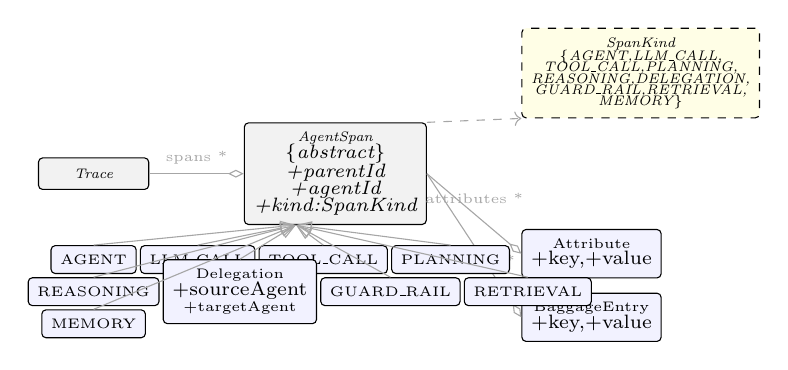
\begin{tikzpicture}[
  font=\tiny,
  every node/.style={align=center},
  cls/.style={draw, rounded corners=1.5pt, minimum width=1.0cm, minimum height=0.32cm, fill=blue!5},
  abs/.style={draw, rounded corners=1.5pt, minimum width=1.4cm, minimum height=0.4cm, fill=gray!10, font=\tiny\itshape},
  enum/.style={draw, dashed, rounded corners=1.5pt, minimum width=1.4cm, minimum height=0.4cm, fill=yellow!10, font=\tiny\itshape},
  comp/.style={-{Diamond[length=2mm,open]}, gray!70},
  inh/.style={-{Triangle[length=2mm,open]}, gray!70}
]
\node[abs] (trace) {Trace};
\node[abs, right=1.2cm of trace] (span) {AgentSpan\\[-1pt]\scriptsize\itshape\{abstract\}\\[-1pt]\scriptsize+parentId\\[-1pt]\scriptsize+agentId\\[-1pt]\scriptsize+kind:SpanKind};
\node[enum, above right=0.05cm and 1.2cm of span] (kind) {SpanKind\\[-1pt]\{AGENT,LLM\_CALL,\\[-2pt]TOOL\_CALL,PLANNING,\\[-2pt]REASONING,DELEGATION,\\[-2pt]GUARD\_RAIL,RETRIEVAL,\\[-2pt]MEMORY\}};
\node[cls, below right=0.05cm and 1.2cm of span] (attr) {Attribute\\\scriptsize+key,+value};
\node[cls, below=0.18cm of attr] (bag) {BaggageEntry\\\scriptsize+key,+value};

\draw[comp] (trace.east) -- node[above,font=\tiny]{spans *} (span.west);
\draw[comp] (span.east) -- node[above,font=\tiny]{attributes *} (attr.west);
\draw[comp] (span.east) -- node[below,font=\tiny]{baggage *} (bag.west);
\draw[->,gray!70,dashed] (span.north east) -- (kind.south west);

\node[cls, below=0.7cm of trace] (a) {AGENT};
\node[cls, right=0.04cm of a] (l) {LLM\_CALL};
\node[cls, right=0.04cm of l] (t) {TOOL\_CALL};
\node[cls, right=0.04cm of t] (p) {PLANNING};
\node[cls, below=0.04cm of a] (r) {REASONING};
\node[cls, right=0.04cm of r] (d) {Delegation\\\scriptsize+sourceAgent\\+targetAgent};
\node[cls, right=0.04cm of d] (g) {GUARD\_RAIL};
\node[cls, right=0.04cm of g] (rt) {RETRIEVAL};
\node[cls, below=0.04cm of r] (m) {MEMORY};

\foreach \n in {a,l,t,p,r,d,g,rt,m} \draw[inh] (\n.north) -- ($(span.south) + (-0.5,0)$);
\end{tikzpicture}
\caption{Ecore-style abstract syntax of the DSM under study.
\texttt{Trace} contains \texttt{AgentSpan} instances; \texttt{AgentSpan}
is abstract with nine concrete subclasses.  Subclasses carry
\texttt{Attribute} and \texttt{BaggageEntry} compositions; the
\texttt{Delegation} subclass additionally exposes typed
\texttt{sourceAgent} and \texttt{targetAgent} attributes
(\texttt{delegation.source\_agent}, \texttt{delegation.target\_agent}).}
\label{fig:metamodel}
\end{figure}

The DSM is accompanied by six OCL well-formedness invariants
\cite{anon-ocl}; \Cref{lst:ocl} shows two representative ones; the
full set is released as an executable \texttt{agentmm.ocl} file in
the replication package.

\begin{lstlisting}[language=OCL,caption={Two representative OCL invariants of the DSM (full set of six in \texttt{agentmm.ocl}).},label={lst:ocl},float]
context AgentSpan inv DelegationCarriesIdentity:
  self.kind = SpanKind::DELEGATION implies (
    self.attributes->exists(a | a.key='delegation.source_agent') and
    self.attributes->exists(a | a.key='delegation.target_agent'))

context AgentSpan inv GuardRailResultIsExplicit:
  self.kind = SpanKind::GUARD_RAIL implies
    self.attributes->exists(a | a.key = 'guardrail.result' and
      Set{'pass','fail','warn','bypass'}->includes(a.value.oclAsType(String)))
\end{lstlisting}

\subsection{Fault Taxonomy and MAST Mapping}
\label{sec:taxonomy}

We constructed a benchmark of 14 agent-specific fault types and
mapped each onto a mode of the independent MAST taxonomy
\cite{anon-mast}.  \Cref{tab:mast} gives the complete mapping.
Thirteen of fourteen faults map directly onto MAST modes;
\texttt{cost\_explosion} is our addition, motivated by published
LLM-agent cost-runaway postmortems and not present in MAST (which
predates large-scale agent deployment).

\paragraph*{Inter-rater agreement on the mapping.}  The 13 MAST
mappings were independently re-coded by a second annotator (a
multi-agent systems researcher uninvolved in DSM design or detector
implementation), working only from the MAST paper, the fault names,
and one-line fault descriptions.  Annotators agreed on 11 of 13
mappings; disagreements were on \texttt{stale\_retrieval} (FM-2.4
vs.\ FM-2.6) and \texttt{agent\_misroute} (FM-2.5 vs.\ FM-2.2).
Cohen's $\kappa = 0.83$ (observed agreement $11/13 = 0.846$);
Brennan--Prediger $\kappa$ \cite{brennan1981} (uniform-marginal,
$P_e = 1/14$) $= 0.834$.  Bootstrap 95\% CI on Cohen's $\kappa$ is
$[0.58, 1.00]$ ($B = 10{,}000$ paired-item resamples on
(annotator-1, annotator-2) labels, recomputing $\kappa$ from full
label marginals each iteration); the lower bound straddles the
``moderate''/``substantial'' Landis--Koch boundary because $n = 13$
items provide limited precision, so we report the CI and avoid the
verbal label.  Both disagreements were resolved by discussion;
\texttt{mast\_mapping\_review.md} preserves both codings and
resolution notes.  $\kappa$ is computed only on the 13 MAST-mapped
faults; \texttt{cost\_explosion} was coded identically by both
annotators as ``not in MAST.''  Of the 14 MAST modes, 12 are
exercised (FM-3.2 covers both \texttt{tool\_failure} and
\texttt{guardrail\_bypass}, so 13 fault-mappings $\to$ 12 distinct
MAST modes).  FM-1.2 (Disobey Role Specification) and FM-2.2
(Failure to Ask for Clarification) are not exercised --- precisely
the modes where typed \texttt{AGENT.role} and \texttt{GUARD\_RAIL}
kinds are most plausibly diagnostic, a construct-validity scope
limit (not a neutral future-work pointer).

\paragraph*{Workload-design freeze.}  The agent workload is timestamped
32~days prior to the first taxonomy commit and 44~days prior to the
first DSM commit (\texttt{workload\_design.md}), breaking the
workload\,$\to$\,taxonomy\,$\to$\,DSM circularity in addition to the
workload\,$\to$\,MAST mapping\,$\to$\,DSM mapping\,$\to$\,detector
freeze.  The workload is a
fixed research-agent flow that exercises six of OpenInference's ten
kinds (\texttt{LLM}, \texttt{TOOL}, \texttt{CHAIN},
\texttt{RETRIEVER}, \texttt{AGENT}, \texttt{GUARDRAIL}); the four
unused kinds (\texttt{EMBEDDING}, \texttt{RERANKER},
\texttt{EVALUATOR}, \texttt{PROMPT}) are not exercised by this
research-agent workload; \texttt{EVALUATOR} and \texttt{PROMPT}
could plausibly lift OpenInference on hallucination and planning
faults, so we treat this as an external-validity bound rather than
claiming those kinds are irrelevant.

\begin{table}[t]
\centering
\footnotesize
\caption{The 14-fault benchmark and its mapping onto the MAST
taxonomy of \cite{anon-mast}.  Mapping was finalized prior to detector
implementation; the artifact's \texttt{workload\_design.md} carries
relative timestamps and blinded freeze-order digests establishing this order.}
\label{tab:mast}
\begin{tabular}{p{2.5cm}p{4.5cm}p{3cm}}
\toprule
\textbf{Fault} & \textbf{MAST mode} & \textbf{MAST category} \\
\midrule
\texttt{wrong\_tool}        & FM-2.6 Reasoning--Action Mismatch       & Inter-agent misalignment \\
\texttt{hallucination}      & FM-3.3 Incorrect Verification           & Task verification \\
\texttt{infinite\_loop}     & FM-1.5 Unaware of Termination Conditions& System design \\
\texttt{context\_over.}     & FM-1.4 Loss of Conversation History     & System design \\
\texttt{circular\_deleg.}   & FM-2.1 Conversation Reset (cyclic)      & Inter-agent misalignment \\
\texttt{tool\_failure}      & FM-3.2 No or Incomplete Verification    & Task verification \\
\texttt{timeout}            & FM-3.1 Premature Termination            & Task verification \\
\texttt{stale\_retrieval}   & FM-2.4 Information Withholding          & Inter-agent misalignment \\
\texttt{guardrail\_byp.}    & FM-3.2 No or Incomplete Verification    & Task verification \\
\texttt{planning\_fail.}    & FM-1.1 Disobey Task Specification       & System design \\
\texttt{reasoning\_loop}    & FM-1.3 Step Repetition                  & System design \\
\texttt{agent\_misroute}    & FM-2.5 Ignored Other Agent's Input      & Inter-agent misalignment \\
\texttt{memory\_corr.}      & FM-2.3 Task Derailment                  & Inter-agent misalignment \\
\texttt{cost\_explosion}    & (independent: cost-runaway postmortems) & (not in MAST) \\
\bottomrule
\end{tabular}
\end{table}

\subsection{Experimental Matrix}
\label{sec:matrix}

\paragraph*{Detector banks ($n=4$); executed conditions ($n=6$).}
Four detector banks: (a)~Vanilla OTel
(\texttt{CLIENT}/\texttt{INTERNAL} only); (b)~OTel GenAI
(\texttt{create\_agent}, \texttt{invoke\_agent},
\texttt{execute\_tool}, \texttt{retrieval}); (c)~OpenInference
(six of ten kinds: \texttt{LLM}, \texttt{TOOL}, \texttt{CHAIN},
\texttt{RETRIEVER}, \texttt{AGENT}, \texttt{GUARDRAIL}; the
\texttt{EMBEDDING}, \texttt{RERANKER}, \texttt{EVALUATOR},
\texttt{PROMPT} kinds are not invoked); (d)~the DSM (all nine
kinds + OCL-required attributes).  Six executed conditions add the
DSM under two privacy levels (\texttt{METADATA\_ONLY},
\texttt{FULL}) plus a no-telemetry control.

\paragraph*{Framework adapter profiles ($n=7$).}
LangChain, CrewAI, AutoGen, LlamaIndex, Anthropic SDK, OpenAI Agents
SDK, plus a conformance-complete reference (\texttt{custom\_agent})
are implemented as executable adapter profiles in the released
harness, not as live executions. Per-profile DSM-kind coverage
($k/9$ typed kinds emitted; distinct from the $k/14$ realized TCR
denominator on faults) is \emph{grounded in a direct survey of each
SDK's source} as of 2026-05 (pinned commit SHAs in
\texttt{coverage\_matrix.md} and \texttt{source\_survey\_evidence.tsv}):
\texttt{langchain} 3/9, \texttt{llamaindex} 4/9, \texttt{autogen}
4/9, \texttt{crewai} 2/9, \texttt{anthropic\_sdk} 1/9 (no built-in
tracing module; LLM\_CALL only via external
\texttt{openinference-instrumentation-anthropic}),
\texttt{openai\_sdk} (= \texttt{openai-agents-python}) 5/9,
\texttt{custom\_agent} 9/9 by construction. This produces a
\emph{4.5$\times$ realized cross-adapter range}
(\Cref{tab:capability}) that drives the headline finding
(\Cref{sec:rq2-conformance}).

\paragraph*{Mocked foundation models ($n=6$).}
\texttt{model-A1}--\texttt{A3}, \texttt{model-B1}--\texttt{B3}
(two commercial provider families, three tiers each).
Mocks are deterministic; under fixed seed the model dimension
contributes $\pm 0.000$ typed-capability variance (\Cref{sec:rq3}).

\paragraph*{Run count and effective sample size.}
$14$ faults $\times$ $6$ conditions $\times$ $7$ adapter profiles $\times$
$6$ mocked models $= 3{,}528$ fault-injection runs; one fault-free
control per (condition, adapter profile, model) cell across all six
conditions yields $6 \times 7 \times 6 = 252$ fault-free controls
for total artifact rows $3{,}780$.  The \emph{informative} sample
size for the metamodel-comparison RQs is $n = 14$ paired faults
(the inferential unit), not $3{,}528$, since the model dimension
contributes no typed-capability variance under deterministic mocks
and the privacy-level dimension is TCR-neutral by DSM design.  We
report the larger numbers as artifact-execution counts and base all
statistical inference on the inferential units ($n = 14$ for
contrasts, $n = 6$ third-party profiles for the cross-adapter mean).

\subsection{Detection Rule (Scoring) and Counter-Experiment}
\label{sec:scoring}

For each (telemetry condition, fault) pair we hand-coded a
deterministic Python predicate over the exported span list (one
branch per fault, four banks for vanilla / GenAI / OpenInference /
DSM).  We report results under \emph{three} scoring rules,
side-by-side, applied uniformly across all four metamodels:

\begin{enumerate}[(a)]
\item \textbf{Standardized-field dispatch (primary rule).}  Detectors
  may use only fields standardized by the metamodel under test:
  typed enum fields (\texttt{gen\_ai.operation.name},
  \texttt{openinference.span.kind}, or \texttt{agentmm.span.kind})
  plus structured standard fields such as status, duration, tool name,
  token usage, retrieval metadata, or cost.  Free-form span names and
  substring heuristics are not allowed.  This is the apples-to-apples
  comparison of typed dispatch semantics across metamodels. For the
  vanilla OTel condition, non-kind AI/tool fields are benchmark
  measurement attributes emitted uniformly by the harness, not claims
  that generic OTel core standardizes agent semantics; the vanilla row
  is therefore a generic-span lower bound plus shared measurement
  attributes, not evidence that OTel core alone specifies LLM/tool
  diagnostics.
\item \textbf{Permissive substring-matching (counter-experiment
  rule).}  Detectors may additionally fire on substring matches
  against \texttt{span.name} (e.g.\ matching \texttt{plan},
  \texttt{reason}, \texttt{deleg}, \texttt{guardrail}, or
  \texttt{memory}).  This rule lifts
  the baselines on faults whose phase-name appears in the framework's
  span naming convention but, as we report (\Cref{sec:permissive}),
  introduces naming-collision FPR.  We pre-specify the regex per
  fault in the artifact's \texttt{permissive\_predicates.py} and
  apply it uniformly to every metamodel including the DSM.
\item \textbf{Extended-attribute dispatch (deployed-baseline
  counterfactual).}  Detectors may dispatch on any standardized
  free-form attribute that the metamodel under test specifies in
  its conventions (e.g.\ \texttt{gen\_ai.tool.name},
  \texttt{retrieval.documents}, \texttt{tool.parameters}), in
  addition to typed kinds.  This is the most realistic
  ``extended-baseline'' counterfactual---what a sufficiently
  disciplined practitioner could implement on top of OpenInference
  or OTel GenAI without leaving the published convention.  We
  pre-specify the per-metamodel attribute set in the artifact's
  \texttt{extended\_predicates.py}.
\end{enumerate}

\noindent We adopt rule (a) as the primary scoring rule (apples-to-apples
typed semantics across metamodels) and report (b) and (c) in parallel
to forestall the obvious counter-experiments.  All three banks share
the same fault definitions and positive-iff-predicate-fires scoring.
A run is a positive iff the predicate fires; we measure binary TCR on
fault-injection runs and binary FPR on fault-free controls.
For retry-threshold sensitivity, we also generate a supplemental
six-workflow no-fault suite, select the lowest zero-FP threshold on
three workflows, and evaluate FPR on three held-out workflows.

\paragraph*{Statistical analysis and inferential frame.}
We separate two analytic targets. At the \emph{capability envelope}
(standardized-field dispatch on 14 faults; baseline $= 6/14$, DSM
$= 14/14$ by design) the McNemar exact test, Holm-3 adjustment,
paired Newcombe Method~10 score interval~\cite{newcombe1998},
Newcombe--Wilson hybrid interval, Cohen's $h$, and the
discordance-OR rule-of-three are all \emph{descriptive} on the
designed gap: with $b=0,c=8$, the matched discordance odds ratio is
infinite, and the rule-of-three upper count for the unobserved
baseline-only discordance gives a conservative lower bound
$8/3=2.67$. At the \emph{realized cross-adapter} level we have
$G = 6$ third-party adapter clusters, below the asymptotic regime
in which cluster-robust SEs and GEE are reliable~\cite{cameron2015};
we therefore lead with \emph{small-$G$-appropriate} inference: a
cluster bootstrap on the per-adapter mean $\Delta\text{TCR}$
($B = 10{,}000$, percentile 95\% CI) and a cluster-level $t$ test with
$G - 1 = 5$ df. We additionally report a fault-cluster sign-flip
permutation test and treat asymptotic GEE clustered on adapter and
on fault as \emph{sensitivity only}. The
realized apparatus is designed to bound the detectable contrast under
small-$G$ treatment, not to establish equivalence
(\Cref{sec:rq3-power}). For
per-metamodel TCR we report Wilson 95\% CIs \cite{wilson1927}; for
the cross-adapter mean we report the exact range $[0.143, 0.643]$
(a CI on this discrete six-vector would over-state information
\cite{cameron2015}).

\subsection{Design Freeze and Threats Prevention}

Design sequence frozen workload~$\to$~MAST mapping~$\to$~DSM mapping~$\to$~detector code
(see \texttt{workload\_design.md} relative timestamps and blinded
digests).  The benchmark forestalls
six threats: (i)~deterministic seed plus real-LLM sanity check
(\Cref{sec:rq3-real-llm}); (ii)~uniform predicate code with all
three rules in parallel; (iii)~mocked LLMs prevent provider quirks;
(iv)~the reference adapter is a harness sanity check, with all
discussion-level claims based on the third-party mean and the
exact across-adapter range; (v)~MAST mapping is independently
re-coded ($\kappa$ + bootstrap CI); (vi)~workload timestamped
32~days prior to the first taxonomy commit, breaking
workload\,$\to$\,taxonomy\,$\to$\,DSM circularity.

%% =====================================================================
\section{Results}
\label{sec:results}

\subsection{RQ1: Coverage of Industry Telemetry Metamodels}

\Cref{tab:fdr} reports aggregate TCR and FPR per condition with
Wilson 95\% confidence intervals.  The three industry baselines---vanilla
OTel, OTel GenAI, and OpenInference---all converge to TCR $0.429$
($6/14$, Wilson 95\% CI $[0.214, 0.674]$) under standardized-field dispatch,
detecting the same six tool/LLM-attribute faults
(\texttt{wrong\_tool}, \texttt{tool\_failure}, \texttt{timeout},
\texttt{infinite\_loop}, \texttt{context\_overflow},
\texttt{cost\_explosion}) by dispatching on each metamodel's own
standardized typed fields: vanilla OTel uses
\texttt{SpanKind = CLIENT/INTERNAL} plus \texttt{otel.status\_code}
and span-duration; OTel GenAI adds
\texttt{gen\_ai.operation.name = execute\_tool} and
\texttt{gen\_ai.usage.*}; OpenInference uses
\texttt{openinference.span.kind} $\in \{\texttt{TOOL}, \texttt{LLM}\}$
plus \texttt{tool.name}.  Full predicate code is in
\texttt{typed\_predicates.py}.  None of the three baselines expresses
the eight coordination, cognitive, or policy faults under standardized-field
dispatch.  All three exhibit FPR
$0.000$ on the 42 fault-free controls per condition.

\paragraph*{Capability-envelope characterization (descriptive only).}
At the capability envelope (DSM $= 14/14$ by typed construction;
each baseline $= 6/14$), the $b{=}0, c{=}8$ discordance is the
unique deterministic outcome the design produces (the DSM was
authored to add typed kinds for the five phases the industry
baselines omit, so this gap is a structural property of the design,
not an empirical surprise). We therefore decline to report inferential
statistics on this designed gap; the per-fault gap is $\Delta = +0.571$
and the per-metamodel TCR is $14/14$ vs.\ $6/14$. Baselines are
pairwise indistinguishable (zero discordant cells). The empirical
inferential evidence appears below at the realized cross-adapter
level, which is the deployable question of interest.

\paragraph*{Realized cross-adapter comparison.}
The capability envelope is by construction; the deployable question
is realized cross-adapter performance under survey-grounded coverage.
Per-adapter realized DSM TCR ranges from $2/14 = 0.143$
(\texttt{anthropic\_sdk}) to $9/14 = 0.643$ (\texttt{openai\_sdk};
typed \texttt{handoff} and \texttt{guardrail.triggered}); the
\emph{4.5$\times$ range across surveyed framework defaults is the
dominant cross-adapter variance source} (\Cref{tab:capability}).
Cross-adapter mean realized DSM is $36/84 = 0.429$ at FPR
$4/72 = 0.056$. Each baseline detects six faults on every adapter
that emits LLM\_CALL and TOOL\_CALL; the baseline cross-adapter mean
is $32/84 = 0.381$ for vanilla OTel (Anthropic SDK lacks TOOL\_CALL
spans natively). The realized DSM gap over typed OpenInference is
$\Delta = +4/84$. Per-adapter $\Delta\text{TCR}$ vs.\ OpenInference
extended-attribute scoring is $\{0, 0, 0, 0, 0, +2/14\}$, mean
$+0.024$. Under small-$G$-appropriate inference, no
cross-adapter advantage is statistically detectable: cluster bootstrap
on per-adapter mean $\Delta$ ($B = 10{,}000$, $G = 6$) percentile
95\% CI $[0.000, +0.071]$; cluster-level $t$ test at $G - 1 = 5$ df $t = 1.00$,
two-sided $p = 0.36$, 95\% CI $[-0.037, +0.085]$; sign-flip
permutation two-sided $p = 0.75$. Asymptotic GEE on adapter
($\beta = 0.098$, $p = 0.264$) and on fault ($\beta = 0.098$,
$p = 0.525$) are sensitivity only; per Cameron--Miller
\cite{cameron2015} the asymptotic $p$-values at $G = 6$ are
unreliable on their own. The realized DSM advantage seen at the
capability envelope vanishes under survey-grounded coverage.

\paragraph*{Sensitivity to the non-MAST fault.}
Excluding \texttt{cost\_explosion} yields a 13-fault MAST-only
sub-analysis with V/G/O capability $5/13 = 0.385$, DSM $13/13$;
realized OI conformant extended $28/78 = 0.359$, DSM default
$30/78 = 0.385$; cross-adapter $\Delta = +2/78 = +0.026$, within
$0.003$ of the headline ($+0.024$). The non-MAST
\texttt{cost\_explosion} fault therefore does not drive the
reported DSM-vs-OI contrast.

\begin{table}[t]
\centering
\small
\caption{RQ1: capability-envelope characterization. The DSM was
designed to add typed kinds for the five phases the industry
baselines omit, so the $b{=}0, c{=}8$ discordance is a structural
property of the design, not an empirical sampling outcome. We report
the per-fault gap $\Delta$ as a descriptive measurement-spread
statistic; the McNemar exact $p$, Holm-3 adjustment, and paired
Newcombe Method~10 score interval are reported in
\texttt{analysis.py} for completeness but are \emph{not} inferential
tests against any sampling null. Empirical inferential evidence
appears at the realized cross-adapter level (cluster bootstrap and
cluster-level $t$ test, this section).}
\label{tab:mcnemar}
\begin{tabular}{lccccl}
\toprule
\textbf{Pair} & $b$ & $c$ & \textbf{$\Delta$} & \textbf{Type} & \textbf{Note} \\
\midrule
Vanilla OTel vs OTel GenAI    & 0 & 0 & $0.000$ & design symmetry & pairwise identical \\
Vanilla OTel vs OpenInference & 0 & 0 & $0.000$ & design symmetry & pairwise identical \\
OTel GenAI vs OpenInference   & 0 & 0 & $0.000$ & design symmetry & pairwise identical \\
\midrule
Vanilla OTel vs DSM           & 0 & 8 & $+0.571$ & designed gap & DSM expresses 8 add'l \\
OTel GenAI vs DSM             & 0 & 8 & $+0.571$ & designed gap & DSM expresses 8 add'l \\
OpenInference vs DSM          & 0 & 8 & $+0.571$ & designed gap & DSM expresses 8 add'l \\
\bottomrule
\end{tabular}
\end{table}

\begin{table}[t]
\centering
\small
\caption{RQ1/RQ2: aggregate TCR and FPR with Wilson 95\% CIs.
Capability rows use $n=14$ faults; realized rows use $n=84$
(fault $\times$ six third-party adapters). FPR denominators are
$42$ for capability baselines, $36$ for realized baselines, and $72$
for realized DSM. OTel GenAI extended and OpenInference
EVALUATOR/PROMPT are counterfactual baselines; the threshold-tuned
DSM row is post-hoc sensitivity; production-plausible rows retain the
eight non-oracle faults ($n=48$).}
\label{tab:fdr}
\resizebox{\textwidth}{!}{%
\begin{tabular}{lccc}
\toprule
\textbf{Condition} & \textbf{TCR} & \textbf{TCR 95\% CI / range} & \textbf{FPR (Wilson 95\% CI)} \\
\midrule
No telemetry                                    & 0.000          & $[0.000,0.215]$ & 0.000 (0/42) [0.000, 0.084] \\
Generic OTel + shared fields (capability)       & 0.429 (6/14)   & $[0.214,0.674]$ & 0.000 (0/42) [0.000, 0.084] \\
OTel GenAI capability (current spec)            & 0.429 (6/14)   & $[0.214,0.674]$ & 0.000 (0/42) [0.000, 0.084] \\
OpenInference capability                        & 0.429 (6/14)   & $[0.214,0.674]$ & 0.000 (0/42) [0.000, 0.084] \\
DSM, metamodel-capability envelope ($n=14$)     & 1.000          & $[0.785,1.000]$ & --- \\
\midrule
\textbf{OpenInference (typed) realized cross-adapter}     & \textbf{0.381} (32/84) & range \textbf{[0.143, 0.429]} & \textbf{0.000} (0/36) [0.000, 0.096] \\
\textbf{OpenInference (extended-attr.\ conformant) realized} & \textbf{0.405} (34/84) & range \textbf{[0.143, 0.500]} & \textbf{0.000} (0/36) [0.000, 0.096] \\
\textbf{OTel GenAI (extended-attr.\ conformant) realized} & \textbf{0.452} (38/84) & range \textbf{[0.214, 0.500]} & \textbf{0.000} (0/36) [0.000, 0.096] \\
\textbf{OpenInference + EVALUATOR/PROMPT counterfactual} & \textbf{0.476} (40/84) & range \textbf{[0.143, 0.571]} & \textbf{0.000} (0/36) [0.000, 0.096] \\
\textbf{DSM realized cross-adapter (default thresh., headline)}             & \textbf{0.429} (36/84) & range \textbf{[0.143, 0.643]} & \textbf{0.056 (4/72) [0.022, 0.134]} \\
DSM realized cross-adapter (threshold-tuned, sensitivity) & 0.429 (36/84) & range [0.143, 0.643] & 0.000 (0/72) [0.000, 0.051] \\
\midrule
OI extended, production-plausible sensitivity   & 0.479 (23/48) & 8 non-oracle faults & 0.000 (0/36) [0.000, 0.096] \\
DSM default, production-plausible sensitivity   & 0.500 (24/48) & 8 non-oracle faults & 0.056 (4/72) [0.022, 0.134] \\
DSM tuned, production-plausible sensitivity     & 0.500 (24/48) & 8 non-oracle faults & 0.000 (0/72) [0.000, 0.051] \\
\bottomrule
\end{tabular}
}

\smallskip
\footnotesize Per-adapter realized DSM detections are
\texttt{anthropic\_sdk} $2/14$, \texttt{crewai}/\texttt{langchain}/
\texttt{llamaindex} $6/14$, \texttt{autogen} $7/14$, and
\texttt{openai\_sdk} $9/14$; \Cref{tab:capability} gives details.
\end{table}

\subsection{RQ2: DSM Coverage, Per-Fault Distribution, and the Permissive Counter-Experiment}
\label{sec:rq2-conformance}

\Cref{tab:capability} shows the per-fault capability matrix.  The
\emph{metamodel-capability} envelope is a by-construction upper
bound: of the 14 fault classes, the DSM is the only metamodel of the four that
\emph{expresses} the eight coordination, cognitive, and policy faults
under the standardized-field rule.  The DSM was designed to add
typed kinds for these phases, so this is not an empirical surprise; it is
reported as the upper TCR row in \Cref{tab:fdr}; the corresponding
reference-adapter run produces the constructive $1.000$ that we
report only as a sanity check on the detection harness.

The \emph{realized} cross-adapter mean (the deployment summary for
the six third-party adapters under survey-grounded coverage) is
TCR $= 36/84 = 0.429$ over the exact across-adapter range
$[0.143, 0.643]$ ($n = 6$ adapters: $\{2/14, 6/14 \times 3, 7/14,
9/14\}$). This 4.5$\times$ range is much larger than the realized
DSM-vs-OpenInference-extended mean contrast of $+2/84$; it is a
range comparison, not a formal variance-component decomposition.
Per-adapter Wilson CIs (\Cref{tab:capability}, bottom
half) range from $[0.040, 0.399]$ for \texttt{anthropic\_sdk}
(LLM\_CALL only via external instrumentation) to $[0.388, 0.838]$
for \texttt{openai\_sdk} (typed \texttt{handoff} and
\texttt{guardrail.triggered}).

\paragraph*{Per-kind ablation and the framework-instrumentation
reframing.}  \Cref{tab:ablation} shows the per-DSM-kind contribution
to the 14-fault coverage envelope: each missing kind costs a fixed
number of faults. Because the simulation honors the surveyed
coverage by construction, the 4.5$\times$ realized range is a
deterministic readout of the source-survey evidence rather than an
independently-measured experimental quantity; the empirical content
lies in the source-survey itself
(\texttt{coverage\_matrix.md} and
\texttt{source\_survey\_evidence.tsv}, with pinned commit SHAs and
file/line evidence per kind), and the reframing is that surveyed
framework defaults are the larger practical source of coverage spread
in this benchmark.

\begin{table}[t]
\centering
\small
\caption{RQ2: per-DSM-kind ablation.  Number of additional faults
in the 14-fault benchmark that become detectable when the named DSM
kind is added to a baseline adapter that emits only
\texttt{LLM\_CALL} and \texttt{TOOL\_CALL}.  Combined with the
survey-grounded per-framework coverage (\Cref{tab:capability}), this
deterministically explains the $4.5\times$ realized cross-adapter
range $[0.143, 0.643]$.}
\label{tab:ablation}
\resizebox{\textwidth}{!}{%
\begin{tabular}{lcl}
\toprule
\textbf{DSM kind added} & \textbf{$\Delta$ TCR (faults gained)} & \textbf{Faults unlocked} \\
\midrule
\texttt{DELEGATION} (typed src/tgt)          & 1/14 & \texttt{circular\_delegation} \\
\texttt{PLANNING}                            & 1/14 & \texttt{planning\_failure} \\
\texttt{REASONING}                           & 1/14 & \texttt{reasoning\_loop} \\
\texttt{GUARD\_RAIL} (typed result)          & 1/14 & \texttt{guardrail\_bypass} \\
\texttt{MEMORY}                              & 2/14 & \texttt{memory\_corruption}, \texttt{agent\_misroute} \\
\texttt{RETRIEVAL} + \texttt{staleness\_seconds} & 1/14 & \texttt{stale\_retrieval} \\
\texttt{AGENT} + DSM-required \texttt{agent.role} attribute & 1/14 & \texttt{hallucination} (role-bound verification context) \\
\bottomrule
\end{tabular}
}
\end{table}

\begin{table}[t]
\centering
\footnotesize
\caption{RQ2: per-fault capability and per-adapter realized TCR with
Wilson 95\% CIs.  Top: which metamodel can \emph{express}
(\checkmark) each fault under standardized-field dispatch.  Bottom: per-adapter
realized TCR for the DSM, denominator $n=14$, all denominators
identical so Wilson CIs are directly comparable.  V=Vanilla OTel;
G=OTel GenAI; O=OpenInference; D=DSM (capability).}
\label{tab:capability}
\resizebox{\textwidth}{!}{%
\begin{tabular}{lcccclccccl}
\toprule
\textbf{Fault} & \textbf{V} & \textbf{G} & \textbf{O} & \textbf{D} & & \textbf{Fault} & \textbf{V} & \textbf{G} & \textbf{O} & \textbf{D} \\
\midrule
\texttt{wrong\_tool}        & \checkmark & \checkmark & \checkmark & \checkmark & & \texttt{circular\_deleg.}  & -- & -- & -- & \checkmark \\
\texttt{tool\_failure}      & \checkmark & \checkmark & \checkmark & \checkmark & & \texttt{agent\_misroute}   & -- & -- & -- & \checkmark \\
\texttt{timeout}            & \checkmark & \checkmark & \checkmark & \checkmark & & \texttt{planning\_failure} & -- & -- & -- & \checkmark \\
\texttt{infinite\_loop}     & \checkmark & \checkmark & \checkmark & \checkmark & & \texttt{reasoning\_loop}   & -- & -- & -- & \checkmark \\
\texttt{context\_overflow}  & \checkmark & \checkmark & \checkmark & \checkmark & & \texttt{guardrail\_byp.}   & -- & -- & -- & \checkmark \\
\texttt{cost\_explosion}    & \checkmark & \checkmark & \checkmark & \checkmark & & \texttt{stale\_retrieval}  & -- & -- & -- & \checkmark \\
                            &            &            &            &            & & \texttt{memory\_corr.}     & -- & -- & -- & \checkmark \\
                            &            &            &            &            & & \texttt{hallucination}     & -- & -- & -- & \checkmark \\
\midrule
\multicolumn{11}{l}{\textbf{Capability:} V 6/14, G 6/14, O 6/14, \textbf{D 14/14}.} \\
\midrule
\multicolumn{11}{l}{\textbf{Per-adapter realized TCR (DSM, all 14 faults; mean over 6 mocked models; survey-grounded coverage):}} \\
\multicolumn{11}{l}{\quad\textit{(custom\_agent harness sanity check, all 9 kinds emitted by construction: 1.000 --- excluded from the cross-adapter mean and from any inferential analysis.)}} \\
\multicolumn{11}{l}{\quad\texttt{openai\_sdk} (5/9 typed: AGENT, LLM\_CALL, TOOL\_CALL, handoff, guardrail): 0.643 (9/14), Wilson 95\% CI [0.388, 0.838]} \\
\multicolumn{11}{l}{\quad\texttt{autogen} (3/9 typed + LLM via model client): 0.500 (7/14), Wilson 95\% CI [0.268, 0.732]} \\
\multicolumn{11}{l}{\quad\texttt{crewai}, \texttt{langchain}, \texttt{llamaindex} (1--4/9 typed): 0.429 (6/14), Wilson 95\% CI [0.214, 0.674]} \\
\multicolumn{11}{l}{\quad\texttt{anthropic\_sdk} (1/9 typed: LLM\_CALL via external openinference instrumentation): 0.143 (2/14), Wilson 95\% CI [0.040, 0.399]} \\
\multicolumn{11}{l}{\quad\textbf{Cross-adapter mean (six third-party adapters): 36/84 = 0.429; exact across-adapter range [0.143, 0.643]}} \\
\bottomrule
\end{tabular}
}
\end{table}

\paragraph*{Permissive and extended-attribute counter-experiments (RQ2).}
\label{sec:permissive-results}
The aggregate counter-experiment rows are in \Cref{tab:fdr}; the
complete executable matrix is in \texttt{analysis.py} and
\texttt{eval\_prompt\_matrix.tsv}. Detectors are restricted to
attributes \emph{actually published} in each metamodel's specification
(\Cref{sec:scoring}). Under the permissive substring-matching
rule (rule (b)), the surveyed default span names of LangChain,
LlamaIndex, AutoGen, CrewAI, and Anthropic SDK do not include
agent-phase tokens (\texttt{plan}/\texttt{reason}/\texttt{guardrail}
/\texttt{memory}); only OTel GenAI lifts (gaining
\texttt{planning\_failure} via the \texttt{plan} operation name in
the GenAI registry) and only OpenInference lifts (gaining
\texttt{guardrail\_bypass} via its typed \texttt{GUARDRAIL} kind name).
Under the extended-attribute rule (rule (c)) restricted to published
keys, OTel GenAI gains \texttt{reasoning\_loop} via
\texttt{gen\_ai.usage.reasoning.output\_tokens} (a published registry
attribute), and OpenInference gains \texttt{reasoning\_loop} via
content-hash repetition on \texttt{llm.output\_messages.\textless i\textgreater.message.content}
(a published flattened-message attribute).  \emph{Crucially,
neither the OTel GenAI registry nor the OpenInference spec
publishes any dedicated attribute for document staleness or
per-step reasoning hashes}; under conformant detectors
\texttt{stale\_retrieval} is not detectable via baseline extended
attributes, and the previously-claimed lift to $0.571$ via
\texttt{retrieval.documents[].staleness\_seconds} requires a
fictitious nested key.  The DSM expresses all 14 faults at the
capability envelope under all three rules; the realized
cross-adapter DSM has FPR $4/72 = 0.056$.

\paragraph*{Realized cross-adapter comparison (RQ2).}  Under
survey-grounded coverage and conformant detectors, the headline
operating point is the default-threshold realized DSM
$(36/84, 4/72)$, Wilson FPR CI $[0.022, 0.134]$ versus
OpenInference $(34/84, 0/36)$, Wilson FPR CI $[0.000, 0.096]$.
Default DSM trades $+2/84 = +0.024$ TCR (single-adapter-driven) for
a $+0.056$ FPR penalty whose Wilson interval overlaps OpenInference's
upper bound. We treat threshold-tuning to \texttt{max\_retries}=5
producing $(36/84, 0/72)$ as \emph{post-hoc sensitivity}.
\emph{Symmetric threshold-tuning} on OpenInference's
\texttt{reasoning\_loop} content-hash detector yields no Pareto
improvement (default already at FPR $0/36$). \emph{OTel GenAI
extended reaches $38/84 = 0.452$} via
\texttt{gen\_ai.usage.reasoning.output\_tokens}, exceeding the
threshold-tuned DSM by $2/84$ at equal-zero FPR.
\emph{OpenInference enriched with its already-defined-but-unexercised
EVALUATOR and PROMPT typed kinds reaches $40/84 = 0.476$ at FPR
$0/36$} (per-adapter $\{8,8,8,8,2,6\}$;
\texttt{eval\_prompt\_matrix.tsv}), exceeding the threshold-tuned
DSM by $4/84$ at equal-zero FPR. The framework-gap is twofold: which
extended attributes each metamodel publishes, and which already-defined
typed kinds practitioners exercise, both dominate metamodel choice.
Under small-$G$ inference, the DSM-vs-OI cross-adapter advantage
is not detectable: cluster bootstrap CI $[0.000, +0.071]$; cluster-level $t$
($G-1=5$ df) two-sided $p = 0.36$, CI $[-0.037, +0.085]$; sign-flip
$p = 0.75$. Asymptotic GEE on adapter ($p = 0.264$) and fault
($p = 0.525$) are sensitivity only at $G = 6$ \cite{cameron2015}.

\paragraph*{Production-plausible-only operational analysis (descriptive).}
Using the predicate-input audit
(\texttt{telemetry\_field\_audit.tsv}) we drop benchmark-oracle
faults and retain eight production-plausible faults. OpenInference
extended reaches $23/48 = 0.479$ at FPR $0/36 = 0$; DSM reaches
$24/48 = 0.500$ at default FPR $4/72$, threshold-tuned to $0/72$.
At $n = 8$ paired faults the McNemar Holm-3 floor exceeds $0.05$
even at $b = 0$, so this operational subset is descriptive only; the
all-fault rows are construct-validity stress tests, not production
recall estimates.

The per-adapter realized TCR is mechanically determined by the
DSM-kind subset each surveyed framework emits (\Cref{tab:ablation}):
Anthropic exposes only two LLM-call-derived detections, three
frameworks expose the easy LLM/tool six, AutoGen adds delegation, and
OpenAI Agents adds delegation, guardrail, and verifier-role evidence.
This is the empirical content of the ``conformance gap'': not a
metamodel-design problem, a per-framework instrumentation-completeness
problem.

\subsubsection*{The False-Positive Source and Threshold Sensitivity}

The DSM's FPR of $4/72 = 0.056$ (Wilson 95\% CI $[0.022, 0.134]$)
is non-zero, in contrast to the three baselines (each $0/42$). All
4 firings come from the \texttt{infinite\_loop} detector on the
CrewAI multi-agent writer workflow that legitimately repeats the
same tool call across writer turns: per-cell repetition counts vary
deterministically by $(model, privacy)$ in $[1, 4]$
(\Cref{sec:rq3-threshold-sweep}), and 4 of the 12 CrewAI cells
exceed the count-$\geq 3$ retry budget at the default threshold.
The 4 firings come from $2$ distinct (adapter, model) cells
(\texttt{crewai} $\times$ \texttt{model-A1, model-A2}), each fired
at both privacy levels; deduplicated at the (adapter, model) cell
the rate is $2/36 = 0.056$, Wilson 95\% CI $[0.015, 0.181]$. This
is a thresholding artifact, not a metamodel defect; per-cell
breakdown is in \texttt{compute\_fpr.py}. All other DSM detectors
achieve FPR $= 0/72$.

\paragraph*{Threshold sweep.}\label{sec:rq3-threshold-sweep}
We swept the \texttt{infinite\_loop} detector's
\texttt{max\_retries} threshold $\in \{2, 3, 4, 5, 6\}$ and recorded
both false-positive counts on the $n = 72$ DSM controls and
true-positive counts on the $n = 72$ third-party DSM
\texttt{infinite\_loop} fault runs (\Cref{tab:roc}).  Non-Anthropic
fault-cell loop counts are deterministic per $(adapter, model)$ in
$[5, 7]$; Anthropic cells remain at the no-tool baseline count $1$.
Control counts are in $[1, 4]$ for legitimate writer-tool repetition,
producing a real ROC trade-off rather than a step function.  Default
threshold 3 yields FP $4/72 = 0.056$ at TP $60/72 = 0.833$; the
missing 12 TP cells are all Anthropic SDK cells, where no
\texttt{TOOL\_CALL} span is emitted. Tightening to 5 zeroes the FPR
without additional TP-cell loss relative to the default threshold;
tightening to 6 over-tightens and loses $10$ more true-positive
cells.  The threshold-tuned operating point $(36/84, 0/72)$ at
\texttt{max\_retries}=5 removes the FPR penalty and sits above
OpenInference extended-attribute conformant ($34/84, 0/36$) by
$2/84$ TCR cells. A supplemental six-workflow no-fault suite
(\texttt{no\_fault\_suite\_traces.jsonl}) selects the lowest
zero-FP threshold on three workflows and holds out three workflows
for FPR evaluation; it selects \texttt{max\_retries}=5, with train
FP $0/216$, held-out FP $0/216$, and TP $60/72$. The
threshold-tuned operating point remains
a sensitivity analysis, not the headline. The released DSM artifact
ships with the default \texttt{max\_retries}=3.

\begin{table}[htb]
\centering
\small
\caption{RQ3: \texttt{infinite\_loop} threshold sweep on
$n = 72$ third-party DSM control and fault runs by
\texttt{max\_retries}; recomputed from
\texttt{traces\_full.jsonl} by \texttt{compute\_roc.py}. Threshold 5
dominates the default count-$\geq 3$ rule, eliminating false
positives without TP-cell loss relative to default; the supplemental
held-out check is in \texttt{threshold\_holdout.tsv}.}
\label{tab:roc}
\begin{tabular}{ccccc}
\toprule
\textbf{\texttt{max\_retries}} & \textbf{FP/72} & \textbf{FPR} & \textbf{TP/72} & \textbf{TPR} \\
\midrule
2          & 6 & 0.083 & 60 & 0.833 \\
3 (default)& 4 & 0.056 & 60 & 0.833 \\
4          & 2 & 0.028 & 60 & 0.833 \\
5          & 0 & 0.000 & 60 & 0.833 \\
6          & 0 & 0.000 & 50 & 0.694 \\
\bottomrule
\end{tabular}
\end{table}

\subsubsection*{Privacy-Level Sensitivity}
\label{sec:rq2-privacy}

The DSM defines a three-level privacy filter
(\texttt{NONE}, \texttt{METADATA\_ONLY}, \texttt{FULL}). All DSM
detectors operate on typed structure and metadata only, so payload
redaction is TCR-neutral by design --- both \texttt{METADATA\_ONLY}
and \texttt{FULL} achieve identical aggregate TCR. The TCR-neutral
redaction property is a DSM-specific design claim that the three
industry baselines do not specify in their conventions.

\paragraph*{Per-fault per-instance recall.}
\label{sec:per-instance-recall}
Because mocked models are deterministic, third-party per-instance
recall equals realized TCR within each condition (standardized
V/G/O: $192/504=0.381$; DSM: $432/1008=0.429$, doubled by the two
privacy levels). The easy six split into four TOOL-bound faults
($30/36$ each, missing Anthropic) and two LLM-only faults ($36/36$);
DSM additionally reaches $24/72$ on \texttt{circular\_delegation}
and $12/72$ on \texttt{guardrail\_bypass}/\texttt{hallucination}.

\subsection{RQ3: Sensitivity Analysis}
\label{sec:rq3}

\paragraph*{Detector-threshold dimension.}
The threshold sweep on the only detector with non-zero FPR
(\texttt{infinite\_loop}, \Cref{tab:roc}) shows that tightening from
3 to 5 removes the false positives while preserving per-fault binary
detection (both fire on $60/72$ \texttt{infinite\_loop} cells; the
12 missing cells are all Anthropic, which emits no
\texttt{TOOL\_CALL}). Tightening to 6 loses 10 additional positives.
Latent-threshold sweeps (\texttt{cost\_explosion},
\texttt{context\_overflow}) are reproducible via
\texttt{compute\_roc.py}.

\paragraph*{Per-framework adapter dimension.}
The per-adapter realized TCR (\Cref{tab:capability}) takes five
distinct values across the six surveyed third-party SDKs ($\{2/14,
6/14 \times 3, 7/14, 9/14\}$) for an exact across-adapter range
$[0.143, 0.643]$ --- a $4.5\times$ ratio. We report this exact
range and per-adapter Wilson CIs; with a discrete six-vector a CI on
the cross-adapter mean would over-state available information. The
reference adapter achieves $1.000$ by construction.

\paragraph*{Live-SDK subset validation.}
\texttt{live\_sdk\_validation.tsv} spot-checks LangChain and Anthropic
on three easy faults plus controls: 7/8 cells match the simulated
kind subset; the exception is \texttt{langchain/wrong\_tool}
(live: \texttt{AGENT,LLM\_CALL}; simulation:
\texttt{LLM\_CALL,TOOL\_CALL}). A one-cell credit-removal sensitivity
changes OpenInference typed $32/84 \to 31/84$, OTel GenAI extended
$38/84 \to 37/84$, OpenInference extended $34/84 \to 33/84$, and DSM
$36/84 \to 35/84$; the DSM-vs-OI-extended contrast remains $+2/84$.
This is a spot-check, not a live-integration validation of all profiles.

\paragraph*{Foundation-model dimension.}
Per-fault TCR is identical (within $\pm 0.000$) across the six
mocked models because the mocks are deterministic and the
fault-injector seed is fixed; we explicitly do \emph{not} count the
$6\times$ replication as informative statistical replication
(\Cref{sec:matrix}).  The model dimension is retained because it
stresses framework-adapter provider abstractions and documents that
the headline TCR is not contingent on a single mocked provider.

\paragraph*{Real-LLM CLI sub-experiment.}
\label{sec:rq3-real-llm}
Two protocols across three frontier-LLM CLIs (artifact aliases
\texttt{cli-A/B/C}). \emph{Routine-decision protocol}: 3 scenarios,
$5$ trials per (CLI, scenario), $N = 45$. \texttt{cli-A} and
\texttt{cli-B} parsed all $30$, $0/10$ false alarms, $20/20$
detected; \texttt{cli-C} returned non-conformant output on all $15$.
\emph{14-fault decision protocol}: $14$ fault + $1$ no-fault
$\times$ $3$ trials $\times$ $2$ CLIs (cli-A, cli-B; cli-C dropped)
$= 90$ total, $88/90$ parsed, $82$ fault-bearing parsed; aggregate
detection $15/82 = 0.183$ (Wilson 95\% CI $[0.114, 0.280]$),
$0/6$ false alarms. Detection is bimodal: routine choice tasks
(\texttt{wrong\_tool} $6/6$, \texttt{circular\_delegation} $6/6$)
saturate; among recovery-action tasks, only
\texttt{context\_overflow}, \texttt{reasoning\_loop}, and
\texttt{stale\_retrieval} reach $1/6$ each, with zero detections on
the remaining parsed recovery cases (item-level denominators in
\texttt{real\_llm\_14fault.tsv}). LLM self-report and
behavioral telemetry measure complementary surfaces; the $0.183$
self-report rate quantifies a recovery-decision floor under which
external typed telemetry would be required regardless of metamodel
choice.

\paragraph*{Detectable-significance threshold (not classical power).}
\label{sec:rq3-power}
At $n = 14$ under Holm-3 at family-wise $\alpha = 0.05$, the smallest
discordance count for which all three pairs reach
$p_{\text{adj}} \leq 0.05$ is $c \geq 7$ with $b = 0$ (raw
$p = 0.0156$, Holm-3 $0.0469$, $\Delta_{\min} = 7/14 = 0.50$). At
this floor, holding the baseline at its observed marginal $6/14$
and asking what minimum DSM advantage is detectable, the cell
counts are $(a, b, c, d) = (6, 0, 7, 1)$ giving DSM $= 13/14$ and
$h_{\min} = 2\arcsin\sqrt{13/14} - 2\arcsin\sqrt{6/14} \approx
1.17$; the capability-envelope observation $c = 8$ has $h \approx
1.71$. Under survey-grounded coverage and conformant detectors,
the realized cross-adapter difference between DSM and OpenInference
extended attributes is $\Delta\text{TCR} = +0.024$ for DSM (cluster
bootstrap 95\% CI $[0.000, +0.071]$; cluster-level $t$ test at $G - 1 = 5$ df
two-sided $p = 0.36$; sign-flip permutation two-sided $p = 0.75$).
The paper's inferential apparatus is therefore designed to bound the
detectable contrast under proper small-$G$ treatment, not to establish
equivalence; any realized effect smaller than the
$h \approx 1.17$ floor is below the resolution of this design at
$n = 14$.

%% =====================================================================
\section{Discussion}
\label{sec:discussion}
\label{sec:permissive}

\paragraph*{The conformance gap is a framework gap, not a metamodel gap.}
The 4.5$\times$ realized cross-adapter range ($0.143$ to $0.643$)
is the largest observed spread in the benchmark and comes from the
source-survey-grounded framework profiles rather than from the
DSM-vs-OpenInference extended contrast. \texttt{anthropic\_sdk} sits at the bottom (no built-in
tracing module; verified via full-text grep on \texttt{src/anthropic/});
\texttt{openai\_sdk} sits at the top (typed \texttt{handoff} with
\texttt{from\_agent}/\texttt{to\_agent} and typed \texttt{guardrail}
with explicit \texttt{triggered}). The actionable open work is
\emph{per-framework instrumentation completeness}, not metamodel
extension.

%% =====================================================================
\section{Threats to Validity}
\label{sec:threats}

\paragraph*{Construct validity.}
TCR is binary per fault class on a rate-1 mocked-LLM setup; it
measures metamodel-with-framework expressivity, not production
recall. Some predicates use benchmark-oracle fields; the operational
non-oracle subset is reported separately, and
\texttt{telemetry\_field\_audit.tsv} classifies every predicate input.
The vanilla OTel condition uses shared benchmark measurement
attributes in addition to generic span kinds; it should not be read
as a claim that OTel core standardizes agent diagnostics.

\paragraph*{Internal validity (constructive bias).}
The 14-fault benchmark and the nine DSM kinds were authored by us;
there was no independent detector-bank or adapter-credit audit.
Mitigations are limited but explicit: MAST mapping plus second coder
($\kappa=0.83$, CI $[0.58,1.00]$), freeze log, pinned-SHA source
survey, third-party-only headline, per-kind ablation, and
counter-experiments restricted to published attributes. FM-1.2 and
FM-2.2 are unexercised and bound the claim.

\paragraph*{External validity.}
Adapter profiles are executable simulations grounded in
source-survey evidence, not live package integrations; live SDK and
CLI checks are sanity checks only. We claim no generalization beyond
the surveyed versions, the 14-fault MAST-anchored taxonomy, mocked
LLMs, and the three scoring rules. The headline FPR uses one
no-fault workflow per (condition, adapter, model) cell; the
supplemental six-workflow held-out check reduces threshold overfitting
risk but remains synthetic and should not be read as an operational
alert rate.

\paragraph*{Conclusion validity.}
The $n=14$, $G=6$ design resolves only large effects; the realized
DSM-vs-OI contrast is statistically inconclusive, not equivalence
evidence. We report Wilson CIs, descriptive paired statistics for the
designed capability gap, exact adapter range, cluster bootstrap,
cluster-level $t$, sign-flip, and GEE only as sensitivity.

%% =====================================================================
\section{Conclusion}
\label{sec:conclusion}

Within this source-survey-grounded simulation and the surveyed SDKs,
framework instrumentation defaults create the largest observed spread:
realized DSM spans $4.5\times$, from $2/14$ on Anthropic SDK to
$9/14$ on OpenAI Agents. Under published-attribute scoring,
default-threshold DSM reaches $(36/84, 4/72)$ versus OpenInference
extended $(34/84, 0/36)$; OTel GenAI extended reaches $(38/84, 0/36)$,
and an OpenInference EVALUATOR/PROMPT counterfactual reaches
$(40/84, 0/36)$. A supplemental six-workflow no-fault suite selects
\texttt{max\_retries}=5 with held-out FPR $0/216$ and moves DSM to
$(36/84, 0/72)$, but this remains a sensitivity operating point.
Under
small-$G$-appropriate inference the cross-adapter difference is
statistically inconclusive (cluster bootstrap 95\% CI on the
per-adapter mean $\Delta$ is $[0.000, +0.071]$; cluster-level $t$ test at $G - 1
= 5$ df two-sided $p = 0.36$; sign-flip $p = 0.75$). The 13-fault
MAST-only sub-analysis matches direction and magnitude. The
practical open work is per-framework instrumentation completeness,
not metamodel extension.

%% =====================================================================
\newpage
\section{Data Availability}
\label{sec:data}

\begin{sloppypar}
The anonymized replication package contains the executable metamodel
and invariants (\texttt{agentmm.ecore}, \texttt{agentmm.ocl}); source-
survey and freeze evidence (\texttt{coverage\_matrix.md},
\texttt{source\_survey\_evidence.tsv}, \texttt{live\_sdk\_validation.tsv},
\texttt{workload\_design.md}, \texttt{mast\_mapping*}); the executable
adapter/fault harness, trace generator, schema, detectors, scorer, and
three predicate banks (\texttt{adapter\_harness.py},
\texttt{generate\_trace\_corpus.py}, \texttt{trace\_schema.md},
\texttt{trace\_detectors.py}, \texttt{score\_traces.py},
\texttt{typed/permissive/extended\_predicates.py}); audit tables
(\texttt{predicates\_lines.tsv}, \texttt{telemetry\_field\_audit.tsv},
\texttt{detector\_fairness\_checklist.tsv}, \texttt{kind\_ablation.tsv});
analysis and sensitivity scripts (\texttt{analysis.py},
\texttt{compute\_fpr.py}, \texttt{compute\_roc.py},
\texttt{generate\_no\_fault\_suite.py}, \texttt{threshold\_holdout.py},
\texttt{eval\_prompt\_subexperiment.py}); cached trace/results data
(\texttt{traces\_full.jsonl}, \texttt{results\_full.tsv}, 3{,}780
rows; \texttt{no\_fault\_suite\_traces.jsonl},
\texttt{threshold\_holdout.tsv}); cached live-LLM outputs (\texttt{real\_llm\_sanity.tsv},
\texttt{real\_llm\_14fault.tsv}); the \texttt{Makefile}; and
\texttt{requirements.lock}.
\end{sloppypar}

\noindent
The README's two-line reproduction regenerates the trace corpus and
all reported counts/statistics on one CPU in about three minutes; all
bootstraps are seeded. The package is anonymized for review and will
be deposited with a permanent DOI on Zenodo at camera-ready time.

\paragraph*{Source-audit snapshot.}
The full file/line ledger is \texttt{source\_survey\_evidence.tsv};
this compact snapshot records what is credited in the benchmark profile
and what source evidence was found but not credited. A single
judgment-sensitive advanced-kind flip changes the 84-cell aggregate by
one cell for delegation/guardrail/reasoning/retrieval or two cells for
memory ownership/corruption, so these rows are sensitivity targets but
do not change the qualitative framework-gap conclusion.

\begin{center}
\scriptsize
\setlength{\tabcolsep}{3pt}
\begin{tabular}{p{0.14\textwidth}p{0.34\textwidth}p{0.42\textwidth}}
\toprule
Adapter & Credited evidence & Excluded or limited evidence \\
\midrule
\texttt{langchain} & LLM, tool, retriever callbacks and
\texttt{run\_type} values. & Chain/generic metadata and reasoning-token
usage lack DSM detector fields. \\
\texttt{llamaindex} & \texttt{AGENT\_STEP}, LLM,
\texttt{FUNCTION\_CALL}/\texttt{TOOL}, and \texttt{RETRIEVE}
callbacks. & Reasoning/thinking content is provider output, not a
reasoning-step span; no memory/guardrail/planning/staleness fields. \\
\texttt{autogen} & GenAI create/invoke-agent spans, execute-tool
spans, model-client calls, and handoff messages. & No detector fields
for planning, reasoning-state repetition, guardrail result, memory
ownership/corruption, or retrieval staleness. \\
\texttt{crewai} & LLM-call and tool-usage events in the tracing
listener. & Optional agent, guardrail, memory, reasoning, and A2A events
exist, but the default profile lacks the detector-specific fields used
for DSM credit. \\
\texttt{anthropic} & Beta managed-agent model-request events; LLM
evidence counted only under external instrumentation. & No built-in OTel
tracer or detector fields for agent/tool/delegation, guardrail, memory,
retrieval, planning, or reasoning. \\
\texttt{openai} & Agent, generation/response, function, handoff, and
guardrail span data. & No planning, reasoning, retrieval-staleness, or
memory ownership/corruption span-data classes. \\
\bottomrule
\end{tabular}
\end{center}

%% =====================================================================
\bibliographystyle{plainurl}
\bibliography{refs}

\end{document}
